\chapter{The Lagrangian as a Code for Field Equations and Interactions}

These notes follow Leonard Susskind's Lecture 9 in \emph{Particle Physics 1: Basic Concepts}, with curation by LazyingArt LLC. The lecture begins from a simple complaint: every field has its own equation of motion, but writing them all separately is a poor way to organize the physics. The Lagrangian is introduced instead as a compact code. First it generates the classical field equations. Then, without changing the symbols very much, it is re-read quantum mechanically as a code for local processes of propagation, emission, absorption, creation, annihilation, and scattering.

\section{Why Field Equations Are Coded by a Lagrangian}

The starting point is familiar. Bosonic fields, fermionic fields, and electromagnetic fields all satisfy equations of motion, and those equations involve derivatives with respect to space and time together with the undifferentiated field itself. One could certainly write down all those equations one by one, but the lecture insists on a more economical viewpoint: there is a single object from which they all follow.

That object is the Lagrangian. Susskind does not pause here to rederive the principle of least action; instead he uses the Lagrangian operationally. It is the compact expression that contains, in condensed form, the dynamics of the whole system.

\begin{figure}[htbp]
\centering

\includegraphics[width=0.82\textwidth]{lecture_09_figure_03.png}
\caption{Lagrangian as a function of fields and derivatives}
\end{figure}

For a single scalar field, the board writes the dependence in the form
\begin{equation}
\mathcal{L}
=
\mathcal{L}\!\left(\phi,\partial_t\phi,\partial_x\phi,\ldots\right)
=
\mathcal{L}\!\left(\phi,\partial_\mu\phi\right).
\end{equation}
The point is pedagogical as much as notational. One first writes the explicit time and space derivatives, and only then compresses them into the relativistic shorthand \(\partial_\mu \phi\).

\section{One Scalar Field: Dependence and the Euler--Lagrange Rule}

Having written down what the Lagrangian depends on, the lecture immediately states the rule that generates the field equation. He is explicit that he is not proving the rule here; he is simply reminding us of it and then moving quickly to examples.

For one field \(\phi\), the field-theory Euler--Lagrange equation is
\begin{equation}
\frac{\partial}{\partial t}\frac{\partial \mathcal L}{\partial \dot\phi}
+
\frac{\partial}{\partial x}\frac{\partial \mathcal L}{\partial \phi_x}
+
\frac{\partial}{\partial y}\frac{\partial \mathcal L}{\partial \phi_y}
+
\frac{\partial}{\partial z}\frac{\partial \mathcal L}{\partial \phi_z}
=
\frac{\partial \mathcal L}{\partial \phi},
\end{equation}
where \(\dot\phi=\partial_t\phi\) and \(\phi_x=\partial_x\phi\), and similarly for \(y\) and \(z\).

The lecture then narrows immediately to the simplest possible scalar field. Its Lagrangian is
\begin{equation}
\mathcal L
=
\frac12 \dot\phi^{\,2}
-
\frac12 (\nabla \phi)^2
-
V(\phi).
\end{equation}
The undifferentiated field appears only through the potential \(V(\phi)\). This is exactly the point emphasized on the board.

\begin{figure}[htbp]
\centering

\includegraphics[width=0.72\textwidth]{lecture_09_figure_04.png}
\caption{Potential term in the scalar-field Lagrangian}
\end{figure}

The frame shows only the right half of the board, so we write the standard completion explicitly. The field equation follows by direct differentiation:
\begin{align}
\frac{\partial \mathcal L}{\partial \dot\phi} &= \dot\phi,
&
\frac{\partial \mathcal L}{\partial \phi_x} &= -\phi_x,
&
\frac{\partial \mathcal L}{\partial \phi_y} &= -\phi_y,
&
\frac{\partial \mathcal L}{\partial \phi_z} &= -\phi_z,
\\
\frac{\partial \mathcal L}{\partial \phi} &= -\frac{\partial V}{\partial \phi}.
\end{align}
Therefore
\begin{equation}
\ddot\phi-\nabla^2\phi=-\frac{\partial V}{\partial\phi}.
\end{equation}

Already one sees the lecture's rhythm. First the abstract rule. Then a concrete scalar Lagrangian. Then the equation of motion. Only after that does he ask what the resulting equation means physically.

\section{Scalar Example: Mass Term, Wave Equation, and Relativistic Dispersion}

The simplest interesting potential is not a constant, which contributes nothing to the equation of motion, and not a linear function, which would make the potential energy unbounded from below. The first interesting case is
\begin{equation}
V(\phi)=\frac12 m^2\phi^2.
\end{equation}
Then
\begin{equation}
\frac{\partial V}{\partial\phi}=m^2\phi,
\end{equation}
and the field equation becomes
\begin{equation}
\ddot\phi-\nabla^2\phi=-m^2\phi.
\end{equation}

Now the lecture makes its first important payoff. Instead of leaving this as a formal wave equation, it asks what relation it implies between energy and momentum. We try a plane wave,
\begin{equation}
\phi(\mathbf x,t)\sim e^{i\omega t-i\mathbf k\cdot \mathbf x}.
\end{equation}
Two time derivatives give \(-\omega^2\phi\), and two spatial derivatives give \(-k^2\phi\), where \(k^2=\mathbf k\cdot \mathbf k\). Substituting into the wave equation,
\begin{equation}
-\omega^2\phi-(-k^2)\phi=-m^2\phi.
\end{equation}
Canceling \(\phi\), we obtain
\begin{equation}
\omega^2-k^2=m^2,
\end{equation}
or equivalently
\begin{equation}
\omega^2=k^2+m^2.
\end{equation}
In units with \(\hbar=c=1\), this is just
\begin{equation}
E^2=p^2+m^2.
\end{equation}
Thus the coefficient \(m\) in the potential is interpreted as the mass of a single quantum of the field.

This is one of the lecture's cleanest moves. A single choice of \(V(\phi)\) does not merely alter the field equation; it puts the relativistic mass shell into the theory.

A brief remark on relativity is inserted at exactly this point. If the Lagrangian is a scalar under Lorentz transformations, then the equations of motion it generates are Lorentz invariant. The minus signs between time and space derivatives are not decorative. They are the field-theory imprint of relativistic signature.

\section{Nonlinearity, Multiple Fields, and Classical Scattering}

The next move is to turn free motion into interaction. Suppose the potential contains a cubic term,
\begin{equation}
V(\phi)\supset g\phi^3.
\end{equation}
Then the right-hand side of the field equation acquires an additional contribution
\begin{equation}
-\frac{\partial}{\partial\phi}(g\phi^3)=-3g\phi^2,
\end{equation}
so that schematically
\begin{equation}
\ddot\phi-\nabla^2\phi=-m^2\phi-3g\phi^2.
\end{equation}

Now the equation is no longer linear. That is the crucial point. For a linear equation, sums of solutions are still solutions, and wave packets simply pass through one another, apart from transient interference. Once the equation becomes nonlinear, that superposition principle fails. Wave packets influence one another, distort, and scatter. In the lecture this is the first classical picture of interaction.

The same point becomes sharper with two fields. Let us introduce two scalar fields, \(\phi\) and \(\rho\), and write
\begin{align}
\mathcal L
&=
\frac12 (\partial_\mu\phi)^2
+
\frac12 (\partial_\mu\rho)^2
-
V(\phi,\rho),
\\
V(\phi,\rho)
&=
\frac12 m^2\phi^2+\frac12 M^2\rho^2+\rho\phi^2.
\end{align}
If the mixed term \(\rho\phi^2\) were absent, the two fields would satisfy two uncoupled wave equations:
\begin{equation}
\ddot\phi-\nabla^2\phi=-m^2\phi,
\qquad
\ddot\rho-\nabla^2\rho=-M^2\rho.
\end{equation}
But once the mixed term is present,
\begin{align}
\ddot\phi-\nabla^2\phi &= -m^2\phi-2\rho\phi,
\\
\ddot\rho-\nabla^2\rho &= -M^2\rho-\phi^2.
\end{align}
The equations are now both coupled and nonlinear. A wave packet of \(\phi\) can scatter a wave packet of \(\rho\), and vice versa. In that sense the interaction term already tells us, at the classical level, that the quanta of the two fields will not simply ignore one another.

This is the lecture's summary of classical field theory in miniature. Quadratic terms govern energy, momentum, and mass. Higher-order terms govern interaction.

\section{Dirac Field and Scalar--Fermion Coupling}

The lecture then shifts to a fermionic example. The Dirac equation is written in a classroom shorthand,
\begin{equation}
i\dot\Psi=i\alpha\frac{\partial\Psi}{\partial x}+m\beta\Psi,
\end{equation}
with the understanding that the spatial derivative term really abbreviates the full sum over spatial directions,
\begin{equation}
i\dot\Psi=i\sum_i \alpha_i\frac{\partial\Psi}{\partial x_i}+m\beta\Psi.
\end{equation}

Here Susskind is quite candid: he does not insist on the exact placement of every \(i\) and every parenthesis. The point is not a polished textbook derivation; it is the persistence of the pattern. There is again an equation of motion, and there is again a Lagrangian that generates it.

\begin{figure}[htbp]
\centering

\includegraphics[width=0.76\textwidth]{lecture_09_figure_05.png}
\caption{Dirac equation and its Lagrangian}
\end{figure}

A cleaned classroom form, close to both transcript and board, is
\begin{equation}
\mathcal L_{\mathrm D}
\sim
i\left(
\Psi^\dagger \frac{\partial\Psi}{\partial t}
+
\Psi^\dagger \alpha \frac{\partial\Psi}{\partial x}
+
m\Psi^\dagger\beta\Psi
\right).
\end{equation}
One should read this cautiously. The lecture itself does not pretend that every sign and factor has been fixed once and for all on the board. What matters is that the Dirac field, no less than the scalar field, is encoded by a Lagrangian.

From here the next move is natural: if we also have a scalar field \(\phi\), then we can couple it to the Dirac field. The lecture first writes a non-Lorentz-invariant sketch, then repairs it by inserting a \(\beta\). The result is a coupling of the form
\begin{equation}
\mathcal L_{\mathrm{int}}\propto \Psi^\dagger \beta \Psi\,\phi.
\end{equation}
This term has exactly the intended meaning. The scalar field can scatter the Dirac field, and the Dirac field can scatter the scalar field. In the Dirac equation there will be an extra term proportional to \(\phi\); in the scalar field equation there will be an extra term proportional to the fermion bilinear.

The lecture even emphasizes the suggestive resemblance
\begin{equation}
m\Psi^\dagger\beta\Psi
\quad \longleftrightarrow \quad
\Psi^\dagger\beta\Psi\,\phi,
\end{equation}
as though the mass parameter \(m\) had been replaced by a scalar field. That remark will matter again at the very end.

\section{From Field Operators to QED Vertices}

Up to this point, the discussion is classical. The large pivot now comes: what do these same terms mean in quantum field theory? The answer is that fields are operator-valued objects built from creation and annihilation operators, and products of fields are therefore local codes for particle processes.

For a scalar field, we think schematically of
\begin{equation}
\phi \sim A^+ + A^-,
\end{equation}
where \(A^+\) creates quanta and \(A^-\) annihilates them. Then \(\phi^3(x)\) contains many kinds of local terms at the same spacetime point \(x\):
\begin{itemize}
\item one particle in, two out;
\item two particles in, one out;
\item three particles created from the point;
\item three particles annihilated at the point.
\end{itemize}
So the same cubic term that classically produced nonlinearity is now re-read as a local menu of quantum processes.

The Dirac field is more delicate because it carries both electron and positron content. In the historical language used in the lecture, \(\Psi\) contains annihilation operators for positive-energy electrons and, after the negative-energy reinterpretation, creation operators for positive-energy positrons. Correspondingly,
\begin{align}
\Psi &\sim C^-_{\text{electron}}(+E)+C^+_{\text{positron}}(+E),
\\
\Psi^\dagger &\sim C^+_{\text{electron}}(+E)+C^-_{\text{positron}}(+E).
\end{align}
These formulas should be read schematically, not as a full mode expansion. Their role in the lecture is to organize the possible processes, not to fix every normalization constant.

The basic interaction of quantum electrodynamics is then written in mixed time-space notation as
\begin{equation}
\mathcal L_{\mathrm{QED,int}}
=
e\left(\Psi^\dagger\Psi\,A_0+\Psi^\dagger\alpha\Psi\cdot\mathbf A\right).
\end{equation}
Here \(A_0\) and \(\mathbf A\) are the time and spatial components of the electromagnetic vector potential, and the whole expression is arranged so as to be a scalar.

\begin{figure}[htbp]
\centering

\includegraphics[width=0.78\textwidth]{lecture_09_figure_06.png}
\caption{Field-operator decomposition and photon-emission sketch}
\end{figure}

Once we multiply out the operator content of \(\Psi^\dagger\), \(\Psi\), and the photon field \(A\), the same local vertex can be read in many ways:
\begin{itemize}
\item an electron emits a photon;
\item an electron absorbs a photon;
\item an electron and a positron annihilate into a photon;
\item a photon produces an electron-positron pair.
\end{itemize}
That is the lecture's point: one local algebraic term contains an entire family of physical processes.

\begin{figure}[htbp]
\centering
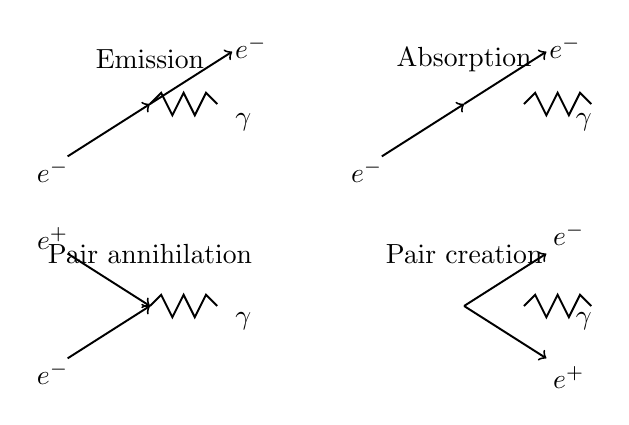
\begin{tikzpicture}[line width=0.7pt, scale=0.95]
\node at (1.2,4.2) {Emission};
\draw[->] (0.1,2.9) -- (1.2,3.6);
\draw[->] (1.2,3.6) -- (2.3,4.3);
\draw (1.2,3.6)--(1.35,3.75)--(1.5,3.45)--(1.65,3.75)--(1.8,3.45)--(1.95,3.75)--(2.1,3.6);
\node at (-0.1,2.7) {$e^-$};
\node at (2.55,4.35) {$e^-$};
\node at (2.45,3.35) {$\gamma$};

\node at (5.4,4.2) {Absorption};
\draw[->] (4.3,2.9) -- (5.4,3.6);
\draw[->] (5.4,3.6) -- (6.5,4.3);
\draw (7.1,3.6)--(6.95,3.75)--(6.8,3.45)--(6.65,3.75)--(6.5,3.45)--(6.35,3.75)--(6.2,3.6);
\node at (4.1,2.7) {$e^-$};
\node at (6.75,4.35) {$e^-$};
\node at (7.0,3.35) {$\gamma$};

\node at (1.2,1.6) {Pair annihilation};
\draw[->] (0.1,0.2) -- (1.2,0.9);
\draw[->] (0.1,1.6) -- (1.2,0.9);
\draw (1.2,0.9)--(1.35,1.05)--(1.5,0.75)--(1.65,1.05)--(1.8,0.75)--(1.95,1.05)--(2.1,0.9);
\node at (-0.1,0.0) {$e^-$};
\node at (-0.1,1.8) {$e^+$};
\node at (2.45,0.7) {$\gamma$};

\node at (5.4,1.6) {Pair creation};
\draw (7.1,0.9)--(6.95,1.05)--(6.8,0.75)--(6.65,1.05)--(6.5,0.75)--(6.35,1.05)--(6.2,0.9);
\draw[->] (5.4,0.9) -- (6.5,1.6);
\draw[->] (5.4,0.9) -- (6.5,0.2);
\node at (7.0,0.7) {$\gamma$};
\node at (6.8,1.85) {$e^-$};
\node at (6.8,-0.05) {$e^+$};
\end{tikzpicture}
\caption{A schematic redraw of the QED vertex family. The same local interaction can be read as emission, absorption, pair annihilation, or pair creation by rotating the legs.}
\end{figure}

All these processes carry the same coefficient \(e\). That coefficient is the electric charge of the electron. In the lecture's microscopic units it is dimensionless, and physically it is interpreted as an amplitude: \(e^2\) sets the probability scale for the basic QED vertex.

Charge conservation appears twice over. Diagrammatically, the fermion arrows must go through the vertex continuously. Algebraically, the interaction contains one \(\Psi\) and one \(\Psi^\dagger\), so whatever \(\Psi\) does to the charge, \(\Psi^\dagger\) undoes.

\subsection{Question \& Answer}

\paragraph{Question.}
If one local QED vertex can be rotated in so many different ways, why do some of the resulting pictures seem to describe impossible processes, such as an electron, positron, and photon all disappearing into nothing?

\paragraph{Answer.}
Because the local vertex is not yet the full amplitude. It is only the local process at a single spacetime point. To obtain a physical amplitude one must integrate over where and when the process takes place. Those spacetime integrals enforce energy and momentum conservation. Once that is done, kinematically forbidden processes simply drop out. So the vertex overgenerates at the local level, but the full spacetime amplitude removes the impossible cases.

\section{Locality, Repeated Action, Symmetry, and the Size of the Full Theory}

The lecture now asks what the quadratic terms mean quantum mechanically. To see it, one replaces a derivative by a finite difference between neighboring points,
\begin{equation}
\partial_x\phi(x)\sim \frac{\phi(x)-\phi(x')}{L},
\end{equation}
where \(x'\) is a nearby point and \(L\) is the separation. Then
\begin{equation}
\frac12\bigl(\partial_x\phi\bigr)^2
\sim
\frac{1}{2L^2}\bigl[\phi(x)-\phi(x')\bigr]^2.
\end{equation}
The same-point pieces describe absorption and re-emission at the same location. The cross-term connects \(x\) and \(x'\): a particle is removed at one neighboring point and re-emitted at the other. This is how the lecture reads the quadratic derivative term as local motion.

The mass term
\begin{equation}
\frac12 m^2\phi^2
\end{equation}
is different. It does not transport the particle. It acts at one point. In the lecture's language, it absorbs a particle and re-emits it from the same point. One may also think of it as a local counting or weighting term. In either reading, it is not motion from one place to another.

\subsection{Question \& Answer}

\paragraph{Question.}
How can a strictly local Lagrangian describe something extended, such as a proton here exchanging a photon with an electron there?

\paragraph{Answer.}
Because there is no single term in the Lagrangian for the whole long-distance process. The exchange is built out of many local steps. One local term emits the photon. Quadratic terms move it from one neighboring point to the next. Another local term absorbs it. In a discrete picture, space or spacetime is divided into tiny cells; the fields live on those cells, and the quadratic terms make particles hop from cell to neighboring cell. The continuum theory is then the limit in which the cells become arbitrarily small.

That is why the lecture insists that there is no action at a distance in quantum field theory. There are only point interactions and infinitesimal hops.

He then gives a useful heuristic for repeated local action. One writes, schematically,
\begin{equation}
\prod_x \bigl(1+\mathcal L_I(x)\bigr),
\end{equation}
where \(\mathcal L_I(x)\) is the interaction part of the Lagrangian at the point \(x\). This expression is explicitly presented as a trick rather than a rigorous final formula, but it captures the combinatorics:
\begin{equation}
(1+\mathcal L_I(x))(1+\mathcal L_I(x'))
=
1+\mathcal L_I(x)+\mathcal L_I(x')+\mathcal L_I(x)\mathcal L_I(x').
\end{equation}
The first term is nothing happening. The next two are single local interactions. The last term is a repeated process at two different points. Multiply enough such factors together and one gets many-step amplitudes built from local ingredients.

Initial and final states fit naturally into this picture. One starts from the vacuum, creates the incoming particles at source points, allows the Lagrangian to act many times in between, and then annihilates the outgoing particles at detector points. The physics between source and detector is exactly what the Lagrangian governs.

The lecture now turns from processes to symmetry. A key example is the global phase transformation
\begin{equation}
\Psi \to e^{i\theta}\Psi,
\qquad
\Psi^\dagger \to e^{-i\theta}\Psi^\dagger,
\qquad
A \to A.
\end{equation}
Because the QED interaction contains equal numbers of \(\Psi\) and \(\Psi^\dagger\), it is unchanged by this transformation. That symmetry is read as charge conservation. In the lecture this is the real utility of the formalism: once the Lagrangian is written, we can read off symmetries, and from symmetries we can read off conservation laws.

As a brief effective-field illustration, the lecture turns to protons, neutrons, and pions. The detailed charge assignments are corrected on the fly, but the cleaned effective vertices are
\begin{equation}
\Psi_p^\dagger\Psi_n\,\pi^+,
\qquad
\Psi_n^\dagger\Psi_p\,\pi^-,
\qquad
\Psi_p^\dagger\Psi_p\,\pi^0,
\qquad
\Psi_n^\dagger\Psi_n\,\pi^0.
\end{equation}
Since the proton is charged, one also has the proton-photon vertex
\begin{equation}
\Psi_p^\dagger\Psi_p\,A.
\end{equation}
The point is not that these are fundamental. The point is that the same bookkeeping applies: a small number of local terms encodes a large family of charge-conserving processes.

At the end the lecture widens out. There is, at least in the physicist's working picture, one huge Lagrangian containing many fields and many couplings. The art is in finding it from experiment. Once it is known, the formalism is precise. In practice one often uses only a small piece of the full Lagrangian, because many sectors of the full theory are irrelevant at a given energy scale. This is why quantum field theory feels at once exact and phenomenological: exact in its rules once the Lagrangian is given, phenomenological in the way that Lagrangian is inferred and truncated.

He closes with a short Higgs-like sketch. Suppose a field \(H\) appears through a term
\begin{equation}
\mathcal L \supset H\phi^2 - V(H).
\end{equation}
If the potential \(V(H)\) has its minimum away from the origin, then in the vacuum
\begin{equation}
\langle H\rangle \neq 0.
\end{equation}
The field \(H\) in the cubic vertex can then be replaced, in the vacuum, by a number. In that sense the cubic interaction begins to look like an effective quadratic mass term. The lecture only gestures at this point, but the idea is clear: a vacuum expectation value can convert interaction structure into mass structure.

\section{Summary}

The lecture develops one idea from beginning to end: the Lagrangian is a compact code. Classically it generates the field equations; quantum mechanically it encodes the elementary local processes from which all amplitudes are built. Quadratic terms govern free propagation and mass, higher powers govern interaction, symmetries govern conservation laws, and extended processes are assembled from repeated local steps. What looks at first like a single formal device turns out to organize almost everything: equations of motion, vertices, locality, charge conservation, and even the way one thinks about the immense and somewhat messy Lagrangian of the world.